\chapter{复数}
\section{复数的概念}
\newpage
\section{复数的几何意义}
\marginnote{2025-4-18}
\subsection{内容分析}
\subsubsection{教材分析}
本节的主要内容包括复平面、复数与点的对应关系、复数与向量的对应关系、复数的模和共轭复数等知识。通过平面直角坐标系中点的坐标与向量的表示,引出复平面与复数的几何意义。

本节内容较为基础,在考试中经常作为题目的一部分与其他知识点结合考查。其中,复数的几何意义与复数的模是考查的重点和热点。

本节内容涉及的主要核心素养包括数学抽象、直观想象、逻辑推理和数学运算。

\subsubsection{学情分析}
在初中阶段,学生已经学习了平面直角坐标系和绝对值的概念,前面还学习了向量的概念与表示,对于数与形的关系已有一定认识。因此,学习复平面与复数的几何意义,学生能够较快进入状态。

然而,学生可能在以下两方面遇到困难:
\begin{enumerate}
    \item 对复数与点的坐标一一对应关系的理解;
    \item 对复数与向量一一对应关系的理解。
\end{enumerate}

\subsubsection{教学目标}
\begin{enumerate}
    \item 理解复数可以用复平面内的点和向量来表示,并掌握它们之间的一一对应关系;
    \item 掌握实轴、虚轴、模等概念,以及用向量的模来表示复数的模的方法;
    \item 通过对复数几何意义的学习,培养学生的数学抽象、数学运算和数学建模等核心素养。
\end{enumerate}

\subsubsection{教学重点与难点}
\begin{itemize}
    \item 教学重点:
          \begin{enumerate}
              \item 正确理解复数的几何意义;
              \item 理解复数的几何意义,并能在复平面内找出复数所对应的点和向量。
          \end{enumerate}
    \item 教学难点:
          \begin{enumerate}
              \item 复数的向量表示;
              \item 理解复数的模和共轭复数的概念,并能运用这些概念解决相关问题。
          \end{enumerate}
\end{itemize}

\subsubsection{教法与学法}
\textbf{教法}:采用启发式教学,通过实例引导学生观察、思考和总结,结合几何图形帮助学生直观理解复数的几何意义。

\textbf{学法}:学生通过自主探究、合作交流和动手作图等方式,理解复数与点、向量的对应关系,掌握复数的模和共轭复数的概念。

\subsubsection{教学案例}
参见《普通高中数学课程标准(2017 年版 2020 年修订)》第 122 页——《案例 10: 复数的引入》。


\subsection{教学设计}
\subsubsection{引入}
\begin{activity}[拆数游戏\cite{CHSX201722006}]
    卡丹的“分 10 问题”:把$10$分成两部分,使其结果分别为$16$,$-24$和$40$,即求解以下方程组:
    \begin{align*}
        1. \begin{cases}
               x+y=10, \\
               xy=16.
           \end{cases}
        \quad
        2. \begin{cases}
               x+y=10, \\
               xy=-24.
           \end{cases}
        \quad
        3. \begin{cases}
               x+y=10, \\
               xy=40.
           \end{cases}
    \end{align*}
\end{activity}

\begin{solution}
    第 1 题和第 2 题类似,这里以第 1 题为例,首先通过消元可得
    \begin{align*}
        x+\frac{16}{x}=10,
    \end{align*}
    进而转化为一元二次方程
    \begin{align*}
        x^2-10x+16=0,
    \end{align*}
    因式分解,即
    \begin{align*}
        (x-2)(x-8)=0,
    \end{align*}
    解得
    \begin{align*}
        x=2 \quad \text{或} \quad x=8,
    \end{align*}
    所以最后有两组对称的解,即
    \begin{align*}
        (x,y)=(2,8) \quad \text{或} \quad (x,y)=(8,2).
    \end{align*}
    第 2 题同理,课堂上可让学生直接通过“瞪眼法”观察得到,重点其实在第 3 题。

    先消元,再配方,得到
    \begin{align*}
        (x-5)^2=-15,
    \end{align*}
    进而
    \begin{align*}
        x = 5\pm\sqrt{-15}.
    \end{align*}
    于是,我们遇到了负数开平方的问题。事实上,这也正是 16 世纪意大利数学家卡丹(G.Cardan,1501—1576)遇到的问题。卡丹是数学史上第一个使用负数平方根的人,不过他称这样的数为“诡辩式”的数,认为他的结果本来就是“不可能”的情形,即使“抛开精神上的痛苦”对它进行运算,依然是“矫揉造作”的。可见他并未完全理解和接受他们。
\end{solution}

\begin{activity}[莱布尼兹的方程]
    对于二元二次方程组:
    \begin{align}
        \begin{cases}
            x^2+y^2=2, \\
            xy=2.
        \end{cases}
        \label{eq:leibniz}
    \end{align}
    求:
    \begin{enumerate}
        \item $x+y$的值;
        \item $x$ 和$y$的值。
    \end{enumerate}
\end{activity}

\begin{solution}
    法一(配凑):$(x+y)^2= x^2+y^2+2xy=6$, 所以$x+y=\pm \sqrt{6}$.

    法二 (消元):由$y=\frac{2}{x}$得$x^2+\frac{4}{x^2}=2$, 进而$x^4-2x^2+4=0$, 令$t=x^2$, 则$t^2-2t+4=0$, 但此时$\Delta=-12<0$, 所有方程无实根,$t$不为实数,$x,y$也不为实数。
\end{solution}

\begin{note}
    从上面的法一则可以进一步得到$x=\sqrt{1+\sqrt{-3}}, y=\sqrt{1-\sqrt{-3}}$ ,从而得到等式 $\sqrt{1+\sqrt{-3}}+\sqrt{1-\sqrt{-3}}=\sqrt{6}$ 。莱布尼茨惊叹道:"在一切分析中,我从来没有见过比这更奇异、更矛盾的事实了。我觉得自己是第一个不通过开方而将虚数形式的根化为实数值的人。"

    因此,历史上数学家并不是因为解一元二次方程而去研究虚数,当一元二次方程的判别式 $\Delta<0$时,方程没有实根,人们采取了"弃之不理"的态度,而是在解三次方程或二元二次方程组时才不得不面对虚数。

    关于法二则可以反问学生,“$x,y$不为实数”就代表方程无解吗?是“无解”还是“无实数解”?进而通过下面的活动进一步研究方程\eqref{eq:leibniz}的解。
\end{note}

\begin{activity}[进一步研究莱布尼茨的方程的解]
    $x^{2}+y^{2}=2$ 是以原点为圆心、$\sqrt{2}$为半径的圆,而 $x y=2$ 是反比例函数。由图象可知两者没有交点,这意味着二元二次方程组\eqref{eq:leibniz}没有实数解。但是,$x+y=\pm \sqrt{6}$ 两条直线是存在的。
    \tikzset{every picture/.style={line width=0.75pt}} %set default line width to 0.75pt        
    \begin{center}

        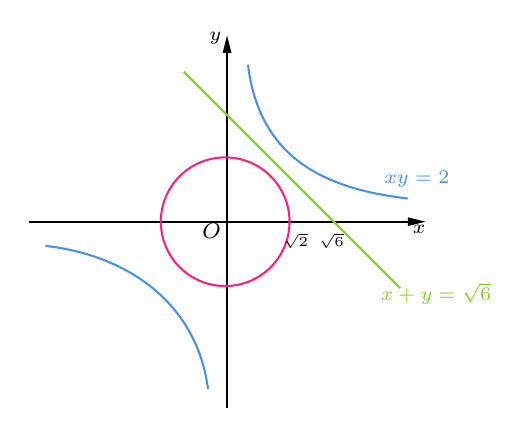
\begin{tikzpicture}[x=0.75pt,y=0.75pt,yscale=-1,xscale=1]
            %uncomment if require: \path (0,300); %set diagram left start at 0, and has height of 300

            %Straight Lines [id:da8026507582116058] 
            \draw    (253,141.76) -- (442.12,141.76) ;
            \draw [shift={(444.12,141.76)}, rotate = 180] [fill={rgb, 255:red, 0; green, 0; blue, 0 }  ][line width=0.08]  [draw opacity=0] (8.4,-2.1) -- (0,0) -- (8.4,2.1) -- cycle    ;
            %Straight Lines [id:da64870239831708] 
            \draw    (348.56,231.5) -- (348.56,54.02) ;
            \draw [shift={(348.56,52.02)}, rotate = 90] [fill={rgb, 255:red, 0; green, 0; blue, 0 }  ][line width=0.08]  [draw opacity=0] (8.4,-2.1) -- (0,0) -- (8.4,2.1) -- cycle    ;
            %Shape: Ellipse [id:dp7551564770874654] 
            \draw  [color={rgb, 255:red, 245; green, 35; blue, 123 }  ,draw opacity=1 ] (316.67,141.76) .. controls (316.67,124.65) and (330.55,110.77) .. (347.66,110.77) .. controls (364.78,110.77) and (378.66,124.65) .. (378.66,141.76) .. controls (378.66,158.88) and (364.78,172.76) .. (347.66,172.76) .. controls (330.55,172.76) and (316.67,158.88) .. (316.67,141.76) -- cycle ;
            %Curve Lines [id:da2129434808692655] 
            \draw [color={rgb, 255:red, 74; green, 144; blue, 226 }  ,draw opacity=1 ]   (358.63,66.12) .. controls (364,109.54) and (393.09,125.65) .. (435.61,130.57) ;
            %Curve Lines [id:da5780763707195247] 
            \draw [color={rgb, 255:red, 74; green, 144; blue, 226 }  ,draw opacity=1 ]   (261.06,153.4) .. controls (300.89,157.88) and (334.01,181.15) .. (339.38,222.33) ;
            %Straight Lines [id:da2981350552987845] 
            \draw [color={rgb, 255:red, 126; green, 211; blue, 33 }  ,draw opacity=1 ]   (327.75,69.48) -- (432.03,173.77) ;

            % Text Node
            \draw (436.55,141.86) node [anchor=north west][inner sep=0.75pt]  [font=\scriptsize]  {$x$};
            % Text Node
            \draw (338.53,48.77) node [anchor=north west][inner sep=0.75pt]  [font=\scriptsize]  {$y$};
            % Text Node
            \draw (335.23,141.09) node [anchor=north west][inner sep=0.75pt]  [font=\footnotesize]  {$O$};
            % Text Node
            \draw (374.19,145.94) node [anchor=north west][inner sep=0.75pt]  [font=\tiny]  {$\sqrt{2}$};
            % Text Node
            \draw (391.4,145.94) node [anchor=north west][inner sep=0.75pt]  [font=\tiny]  {$\sqrt{6}$};
            % Text Node
            \draw (421.19,169.63) node [anchor=north west][inner sep=0.75pt]  [font=\scriptsize,color={rgb, 255:red, 126; green, 211; blue, 33 }  ,opacity=1 ]  {$x+y=\sqrt{6}$};
            % Text Node
            \draw (422.82,115.79) node [anchor=north west][inner sep=0.75pt]  [font=\scriptsize,color={rgb, 255:red, 74; green, 144; blue, 226 }  ,opacity=1 ]  {$xy=2$};


        \end{tikzpicture}
    \end{center}
    根据图象可知, $(x, y)$ 这个点不存在,但其横坐标和纵坐标之和却等于一个实数,两者是存在"矛盾"的。那么问题的关键在哪里?由此从数与形两方面引发学生的认知冲突,让学生面对一种无法弃之不理的"矛盾",从而揭示了引入虚数概念的必要性,虚数的产生变得自然而然。但接下来要解决的问题是如何用几何方式表示复数?
\end{activity}



\subsubsection{新知探究}
1. 复平面

首先,类比实数与数轴上的点一一对应的关系,得到复数与有序实数对对应,而有序实数对又与平面直角坐标系中的点一一对应,所以就可以用平面直角坐标系的点来表示复数。由此介绍复平面、实轴、虚轴等概念。
\begin{itemize}
    \item 实数 $\overset{\text{\tiny 一一对应}}{\longleftrightarrow}$ 数轴上的点
    \item 复数 $\overset{\text{\tiny 一一对应}}{\longleftrightarrow}$ 有序数对 $\overset{\text{\tiny 一一对应}}{\longleftrightarrow}$ 平面直角坐标系上的点
\end{itemize}
\begin{center}

    \tikzset{every picture/.style={line width=0.75pt}} %set default line width to 0.75pt        

    \begin{tikzpicture}[x=0.75pt,y=0.75pt,yscale=-1,xscale=1]
        %uncomment if require: \path (0,300); %set diagram left start at 0, and has height of 300

        %Straight Lines [id:da8790298405518127] 
        \draw    (269,210.55) -- (439.59,210.55) ;
        \draw [shift={(441.59,210.55)}, rotate = 180] [fill={rgb, 255:red, 0; green, 0; blue, 0 }  ][line width=0.08]  [draw opacity=0] (8.4,-2.1) -- (0,0) -- (8.4,2.1) -- cycle    ;
        %Straight Lines [id:da3627886755157933] 
        \draw    (288.92,236.5) -- (288.92,76.42) ;
        \draw [shift={(288.92,74.42)}, rotate = 90] [fill={rgb, 255:red, 0; green, 0; blue, 0 }  ][line width=0.08]  [draw opacity=0] (8.4,-2.1) -- (0,0) -- (8.4,2.1) -- cycle    ;

        %Straight Lines [id:da11661138449086306] 
        \draw [color={rgb, 255:red, 74; green, 144; blue, 226 }  ,draw opacity=1 ] [dash pattern={on 4.5pt off 4.5pt}]  (289.54,120.29) -- (376.24,120.29) ;
        %Straight Lines [id:da8924510381864514] 
        \draw [color={rgb, 255:red, 74; green, 144; blue, 226 }  ,draw opacity=1 ] [dash pattern={on 4.5pt off 4.5pt}]  (376.24,121.58) -- (376.24,210.09) ;
        %Shape: Circle [id:dp8595306873997957] 
        \draw  [fill={rgb, 255:red, 0; green, 0; blue, 0 }  ,fill opacity=1 ] (374.94,120.29) .. controls (374.94,119.57) and (375.52,118.99) .. (376.24,118.99) .. controls (376.96,118.99) and (377.54,119.57) .. (377.54,120.29) .. controls (377.54,121) and (376.96,121.58) .. (376.24,121.58) .. controls (375.52,121.58) and (374.94,121) .. (374.94,120.29) -- cycle ;

        % Text Node
        \draw (275.8,213.46) node [anchor=north west][inner sep=0.75pt]  [font=\footnotesize]  {$O$};
        % Text Node
        \draw (279.28,71.03) node [anchor=north west][inner sep=0.75pt]  [font=\scriptsize]  {$y$};
        % Text Node
        \draw (382.94,102.47) node [anchor=north west][inner sep=0.75pt]    {$Z( a,b)$};
        % Text Node
        \draw (370.69,211.53) node [anchor=north west][inner sep=0.75pt]    {$a$};
        % Text Node
        \draw (274.97,113.76) node [anchor=north west][inner sep=0.75pt]    {$b$};
        % Text Node
        \draw (436.68,213.19) node [anchor=north west][inner sep=0.75pt]  [font=\scriptsize]  {$x$};
        % Text Node
        \draw (422.26,229.22) node [anchor=north west][inner sep=0.75pt]   [align=left] {(实轴)};
        % Text Node
        \draw (232,69.67) node [anchor=north west][inner sep=0.75pt]   [align=left] {(虚轴)};


    \end{tikzpicture}

\end{center}

其中,实轴上的点都表示实数;除了原点外,虚轴上的点都表示纯虚数。

进一步地,因为起点为原点的平面向量与平面直角坐标系中每一个点是一一对应的,所以复数也可以用平面向量来表示。
\begin{center}


    \tikzset{every picture/.style={line width=0.75pt}} %set default line width to 0.75pt        

    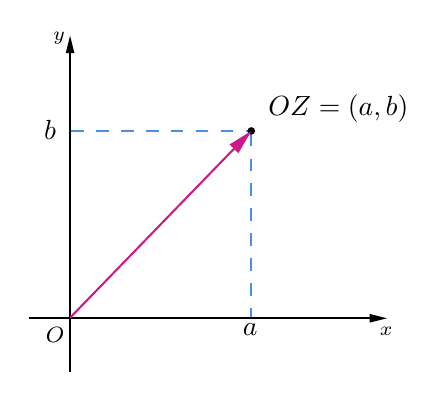
\begin{tikzpicture}[x=0.75pt,y=0.75pt,yscale=-1,xscale=1]
        %uncomment if require: \path (0,300); %set diagram left start at 0, and has height of 300

        %Straight Lines [id:da9506260198545818] 
        \draw    (269,210.55) -- (439.59,210.55) ;
        \draw [shift={(441.59,210.55)}, rotate = 180] [fill={rgb, 255:red, 0; green, 0; blue, 0 }  ][line width=0.08]  [draw opacity=0] (8.4,-2.1) -- (0,0) -- (8.4,2.1) -- cycle    ;
        %Straight Lines [id:da10900803625553457] 
        \draw    (288.92,236.5) -- (288.92,76.42) ;
        \draw [shift={(288.92,74.42)}, rotate = 90] [fill={rgb, 255:red, 0; green, 0; blue, 0 }  ][line width=0.08]  [draw opacity=0] (8.4,-2.1) -- (0,0) -- (8.4,2.1) -- cycle    ;

        %Straight Lines [id:da4613502086281518] 
        \draw [color={rgb, 255:red, 74; green, 144; blue, 226 }  ,draw opacity=1 ] [dash pattern={on 4.5pt off 4.5pt}]  (289.54,120.29) -- (376.24,120.29) ;
        %Straight Lines [id:da9023066685141495] 
        \draw [color={rgb, 255:red, 74; green, 144; blue, 226 }  ,draw opacity=1 ] [dash pattern={on 4.5pt off 4.5pt}]  (376.24,121.58) -- (376.24,210.09) ;
        %Shape: Circle [id:dp4067287412354563] 
        \draw  [fill={rgb, 255:red, 0; green, 0; blue, 0 }  ,fill opacity=1 ] (374.94,120.29) .. controls (374.94,119.57) and (375.52,118.99) .. (376.24,118.99) .. controls (376.96,118.99) and (377.54,119.57) .. (377.54,120.29) .. controls (377.54,121) and (376.96,121.58) .. (376.24,121.58) .. controls (375.52,121.58) and (374.94,121) .. (374.94,120.29) -- cycle ;
        %Straight Lines [id:da6206890372549287] 
        \draw [color={rgb, 255:red, 204; green, 26; blue, 137 }  ,draw opacity=1 ][fill={rgb, 255:red, 0; green, 0; blue, 0 }  ,fill opacity=1 ]   (289,210.2) -- (374.85,121.72) ;
        \draw [shift={(376.24,120.29)}, rotate = 134.14] [fill={rgb, 255:red, 204; green, 26; blue, 137 }  ,fill opacity=1 ][line width=0.08]  [draw opacity=0] (12,-3) -- (0,0) -- (12,3) -- cycle    ;

        % Text Node
        \draw (275.8,213.46) node [anchor=north west][inner sep=0.75pt]  [font=\footnotesize]  {$O$};
        % Text Node
        \draw (279.28,71.03) node [anchor=north west][inner sep=0.75pt]  [font=\scriptsize]  {$y$};
        % Text Node
        \draw (382.94,101.47) node [anchor=north west][inner sep=0.75pt]    {$\lvec{OZ}=( a,b)$};
        % Text Node
        \draw (370.69,211.53) node [anchor=north west][inner sep=0.75pt]    {$a$};
        % Text Node
        \draw (274.97,113.76) node [anchor=north west][inner sep=0.75pt]    {$b$};
        % Text Node
        \draw (436.68,213.19) node [anchor=north west][inner sep=0.75pt]  [font=\scriptsize]  {$x$};


    \end{tikzpicture}
\end{center}

这样我们就得到了复数两种等价的几何意义:
\tikzset{every picture/.style={line width=0.75pt}} %set default line width to 0.75pt        
\begin{center}
    \begin{tikzpicture}[x=0.75pt,y=0.75pt,yscale=-1,xscale=1]
        %uncomment if require: \path (0,300); %set diagram left start at 0, and has height of 300


        % Text Node
        \draw (140.99,185.05) node [anchor=north west][inner sep=0.75pt]   [align=left] {复平面上的点$Z( a,b)$};
        % Text Node
        \draw (426.27,187.72) node [anchor=north west][inner sep=0.75pt]   [align=left] {平面向量$\lvec{OZ}=(a,b)$};
        % Text Node
        \draw (327.42,161.12) node [anchor=north west][inner sep=0.75pt]   [align=left] {\textit{一一对应}};
        % Text Node
        \draw (304.67,96.73) node [anchor=north west][inner sep=0.75pt]    {复数$z=a+b\mathrm{i}$};
        % Connection
        \draw    (295.98,198.03) -- (421.27,197.22) ;
        \draw [shift={(423.27,197.21)}, rotate = 179.63] [fill={rgb, 255:red, 0; green, 0; blue, 0 }  ][line width=0.08]  [draw opacity=0] (12,-3) -- (0,0) -- (12,3) -- cycle    ;
        \draw [shift={(293.99,198.04)}, rotate = 359.63] [fill={rgb, 255:red, 0; green, 0; blue, 0 }  ][line width=0.08]  [draw opacity=0] (12,-3) -- (0,0) -- (12,3) -- cycle    ;
        % Connection
        \draw    (338.75,116.33) -- (243.78,179.94) ;
        \draw [shift={(242.12,181.05)}, rotate = 326.19] [color={rgb, 255:red, 0; green, 0; blue, 0 }  ][line width=0.75]    (10.93,-3.29) .. controls (6.95,-1.4) and (3.31,-0.3) .. (0,0) .. controls (3.31,0.3) and (6.95,1.4) .. (10.93,3.29)   ;
        % Connection
        \draw    (375.12,116.33) -- (477.1,182.63) ;
        \draw [shift={(478.77,183.72)}, rotate = 213.03] [color={rgb, 255:red, 0; green, 0; blue, 0 }  ][line width=0.75]    (10.93,-3.29) .. controls (6.95,-1.4) and (3.31,-0.3) .. (0,0) .. controls (3.31,0.3) and (6.95,1.4) .. (10.93,3.29)   ;

    \end{tikzpicture}
\end{center}

2. 复数的模/绝对值

$|z|=|a+b\mathrm{i}|=\sqrt{a^2+b^2}$, 其中 $a, b \in \mathbb{R}$.

3. 共轭复数(参见书本 p71 例 2)

(1) 定义:$z=a+b\mathrm{i}$与$\overline{z}=a-b\mathrm{i}$互为共轭复数。

(2) 几何意义:$z$和$\overline{z}$关于实轴对称。

(3) 性质(看情况补充):
1. $|z|^2=z\overline{z}$;
2. $\overline{z_1+z_2}=\overline{z_1}+\overline{z_2}$;
3. $\overline{z_1 z_2}=\overline{z_1}\cdot\overline{z_2}$;
4. $\overline{\overline{z}}=z$.

\subsubsection{巩固练习}
\begin{example}[改编自书本 p72 例 3]
    设 $z\in \mathbb{C}$,在复平面内对应的点为$Z$,那么满足下列条件的点$Z$的集合是什么图形?
    \begin{enumerate}
        \item $|z|=1$;
        \item $|z|\leqslant 1$;
        \item $|z|< 1$;
        \item $1<|z|\leqslant 2$.
    \end{enumerate}
\end{example}
\begin{solution}
    如图所示,需注意是是圆周还是圆盘,以及边界是否包含在其中。
    \begin{center}


        \tikzset{every picture/.style={line width=0.75pt}} %set default line width to 0.75pt        

        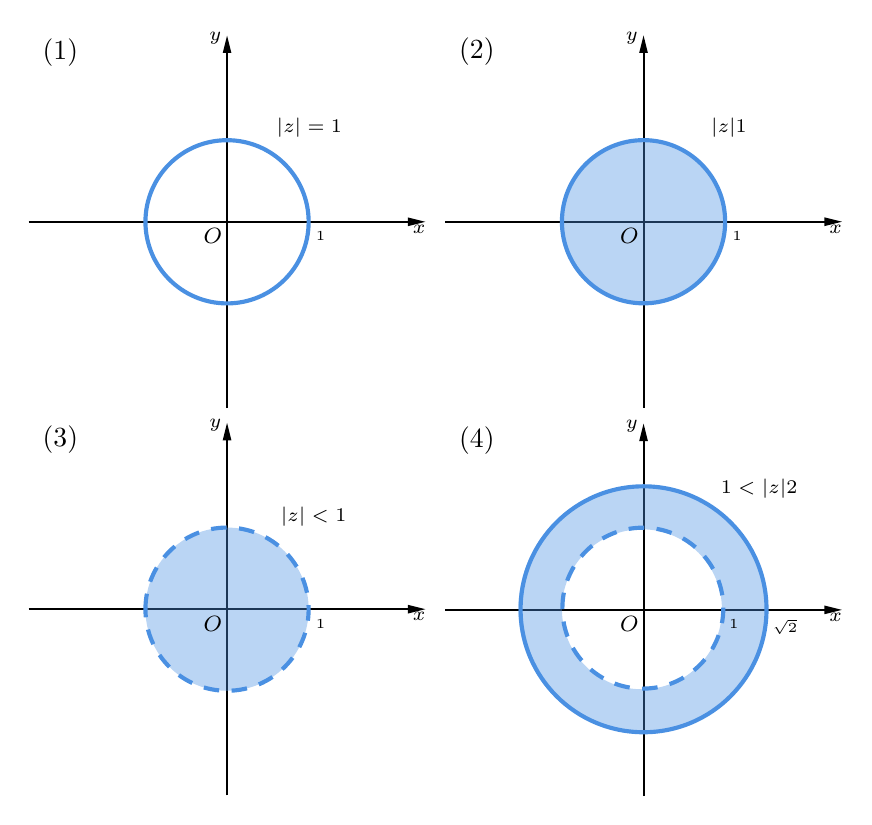
\begin{tikzpicture}[x=0.75pt,y=0.75pt,yscale=-1,xscale=1]
            %uncomment if require: \path (0,498); %set diagram left start at 0, and has height of 498

            %Straight Lines [id:da48952535452117174] 
            \draw    (123.67,111.1) -- (312.78,111.1) ;
            \draw [shift={(314.78,111.1)}, rotate = 180] [fill={rgb, 255:red, 0; green, 0; blue, 0 }  ][line width=0.08]  [draw opacity=0] (8.4,-2.1) -- (0,0) -- (8.4,2.1) -- cycle    ;
            %Straight Lines [id:da7000917064401612] 
            \draw    (219.23,200.84) -- (219.23,23.36) ;
            \draw [shift={(219.23,21.36)}, rotate = 90] [fill={rgb, 255:red, 0; green, 0; blue, 0 }  ][line width=0.08]  [draw opacity=0] (8.4,-2.1) -- (0,0) -- (8.4,2.1) -- cycle    ;
            %Shape: Ellipse [id:dp6427466175006243] 
            \draw  [color={rgb, 255:red, 74; green, 144; blue, 226 }  ,draw opacity=1 ][line width=1.5]  (179.91,111.1) .. controls (179.91,89.38) and (197.51,71.78) .. (219.23,71.78) .. controls (240.94,71.78) and (258.54,89.38) .. (258.54,111.1) .. controls (258.54,132.81) and (240.94,150.42) .. (219.23,150.42) .. controls (197.51,150.42) and (179.91,132.81) .. (179.91,111.1) -- cycle ;
            %Straight Lines [id:da7012394429936882] 
            \draw    (324.33,111.06) -- (513.45,111.06) ;
            \draw [shift={(515.45,111.06)}, rotate = 180] [fill={rgb, 255:red, 0; green, 0; blue, 0 }  ][line width=0.08]  [draw opacity=0] (8.4,-2.1) -- (0,0) -- (8.4,2.1) -- cycle    ;
            %Straight Lines [id:da1521962743776154] 
            \draw    (419.89,200.8) -- (419.89,23.32) ;
            \draw [shift={(419.89,21.32)}, rotate = 90] [fill={rgb, 255:red, 0; green, 0; blue, 0 }  ][line width=0.08]  [draw opacity=0] (8.4,-2.1) -- (0,0) -- (8.4,2.1) -- cycle    ;
            %Shape: Ellipse [id:dp8009519989013992] 
            \draw  [color={rgb, 255:red, 74; green, 144; blue, 226 }  ,draw opacity=1 ][fill={rgb, 255:red, 74; green, 144; blue, 226 }  ,fill opacity=0.38 ][line width=1.5]  (380.57,111.06) .. controls (380.57,89.35) and (398.18,71.75) .. (419.89,71.75) .. controls (441.61,71.75) and (459.21,89.35) .. (459.21,111.06) .. controls (459.21,132.78) and (441.61,150.38) .. (419.89,150.38) .. controls (398.18,150.38) and (380.57,132.78) .. (380.57,111.06) -- cycle ;
            %Straight Lines [id:da04562857260938191] 
            \draw    (123.67,297.73) -- (312.78,297.73) ;
            \draw [shift={(314.78,297.73)}, rotate = 180] [fill={rgb, 255:red, 0; green, 0; blue, 0 }  ][line width=0.08]  [draw opacity=0] (8.4,-2.1) -- (0,0) -- (8.4,2.1) -- cycle    ;
            %Straight Lines [id:da12411551232842866] 
            \draw    (219.23,387.47) -- (219.23,209.99) ;
            \draw [shift={(219.23,207.99)}, rotate = 90] [fill={rgb, 255:red, 0; green, 0; blue, 0 }  ][line width=0.08]  [draw opacity=0] (8.4,-2.1) -- (0,0) -- (8.4,2.1) -- cycle    ;
            %Shape: Ellipse [id:dp9648039203988316] 
            \draw  [color={rgb, 255:red, 74; green, 144; blue, 226 }  ,draw opacity=1 ][fill={rgb, 255:red, 74; green, 144; blue, 226 }  ,fill opacity=0.38 ][dash pattern={on 5.63pt off 4.5pt}][line width=1.5]  (179.91,297.73) .. controls (179.91,276.02) and (197.51,258.41) .. (219.23,258.41) .. controls (240.94,258.41) and (258.54,276.02) .. (258.54,297.73) .. controls (258.54,319.45) and (240.94,337.05) .. (219.23,337.05) .. controls (197.51,337.05) and (179.91,319.45) .. (179.91,297.73) -- cycle ;
            %Straight Lines [id:da5391729869714962] 
            \draw    (324.33,298.06) -- (513.45,298.06) ;
            \draw [shift={(515.45,298.06)}, rotate = 180] [fill={rgb, 255:red, 0; green, 0; blue, 0 }  ][line width=0.08]  [draw opacity=0] (8.4,-2.1) -- (0,0) -- (8.4,2.1) -- cycle    ;
            %Straight Lines [id:da2784087258564013] 
            \draw    (419.89,387.8) -- (419.89,210.32) ;
            \draw [shift={(419.89,208.32)}, rotate = 90] [fill={rgb, 255:red, 0; green, 0; blue, 0 }  ][line width=0.08]  [draw opacity=0] (8.4,-2.1) -- (0,0) -- (8.4,2.1) -- cycle    ;
            %Shape: Donut [id:dp063216757672522] 
            \draw  [color={rgb, 255:red, 0; green, 0; blue, 0 }  ,draw opacity=0 ][fill={rgb, 255:red, 74; green, 144; blue, 226 }  ,fill opacity=0.38 ,even odd rule] (380.57,297.79) .. controls (380.57,276.5) and (397.83,259.25) .. (419.11,259.25) .. controls (440.4,259.25) and (457.65,276.5) .. (457.65,297.79) .. controls (457.65,319.07) and (440.4,336.32) .. (419.11,336.32) .. controls (397.83,336.32) and (380.57,319.07) .. (380.57,297.79)(359.59,297.79) .. controls (359.59,264.91) and (386.24,238.26) .. (419.11,238.26) .. controls (451.99,238.26) and (478.63,264.91) .. (478.63,297.79) .. controls (478.63,330.66) and (451.99,357.31) .. (419.11,357.31) .. controls (386.24,357.31) and (359.59,330.66) .. (359.59,297.79) ;
            %Shape: Ellipse [id:dp07345428958267963] 
            \draw  [color={rgb, 255:red, 74; green, 144; blue, 226 }  ,draw opacity=1 ][line width=1.5]  (360.65,297.79) .. controls (360.65,265.07) and (387.17,238.54) .. (419.89,238.54) .. controls (452.61,238.54) and (479.14,265.07) .. (479.14,297.79) .. controls (479.14,330.51) and (452.61,357.03) .. (419.89,357.03) .. controls (387.17,357.03) and (360.65,330.51) .. (360.65,297.79) -- cycle ;
            %Shape: Ellipse [id:dp08448019654683137] 
            \draw  [color={rgb, 255:red, 74; green, 144; blue, 226 }  ,draw opacity=1 ][fill={rgb, 255:red, 255; green, 255; blue, 255 }  ,fill opacity=0 ][dash pattern={on 5.63pt off 4.5pt}][line width=1.5]  (380.79,297.24) .. controls (380.79,275.83) and (398.15,258.47) .. (419.56,258.47) .. controls (440.98,258.47) and (458.33,275.83) .. (458.33,297.24) .. controls (458.33,318.65) and (440.98,336.01) .. (419.56,336.01) .. controls (398.15,336.01) and (380.79,318.65) .. (380.79,297.24) -- cycle ;

            % Text Node
            \draw (507.88,111.16) node [anchor=north west][inner sep=0.75pt]  [font=\scriptsize]  {$x$};
            % Text Node
            \draw (409.86,18.07) node [anchor=north west][inner sep=0.75pt]  [font=\scriptsize]  {$y$};
            % Text Node
            \draw (407.07,112.89) node [anchor=north west][inner sep=0.75pt]  [font=\footnotesize]  {$O$};
            % Text Node
            \draw (461.21,114.46) node [anchor=north west][inner sep=0.75pt]  [font=\tiny]  {$1$};
            % Text Node
            \draw (329.56,21.14) node [anchor=north west][inner sep=0.75pt]   [align=left] {(2)};
            % Text Node
            \draw (241.67,59.73) node [anchor=north west][inner sep=0.75pt]  [font=\scriptsize]  {$| z| =1$};
            % Text Node
            \draw (451,59.73) node [anchor=north west][inner sep=0.75pt]  [font=\scriptsize]  {$| z| \leqslant 1$};
            % Text Node
            \draw (243.67,247.07) node [anchor=north west][inner sep=0.75pt]  [font=\scriptsize]  {$| z| < 1$};
            % Text Node
            \draw (455.67,233.73) node [anchor=north west][inner sep=0.75pt]  [font=\scriptsize]  {$1< | z| \leqslant 2$};
            % Text Node
            \draw (307.22,297.83) node [anchor=north west][inner sep=0.75pt]  [font=\scriptsize]  {$x$};
            % Text Node
            \draw (209.2,204.73) node [anchor=north west][inner sep=0.75pt]  [font=\scriptsize]  {$y$};
            % Text Node
            \draw (206.4,299.55) node [anchor=north west][inner sep=0.75pt]  [font=\footnotesize]  {$O$};
            % Text Node
            \draw (260.54,301.13) node [anchor=north west][inner sep=0.75pt]  [font=\tiny]  {$1$};
            % Text Node
            \draw (128.89,207.8) node [anchor=north west][inner sep=0.75pt]   [align=left] {(3)};
            % Text Node
            \draw (507.88,298.16) node [anchor=north west][inner sep=0.75pt]  [font=\scriptsize]  {$x$};
            % Text Node
            \draw (409.86,205.07) node [anchor=north west][inner sep=0.75pt]  [font=\scriptsize]  {$y$};
            % Text Node
            \draw (407.07,299.89) node [anchor=north west][inner sep=0.75pt]  [font=\footnotesize]  {$O$};
            % Text Node
            \draw (459.65,301.19) node [anchor=north west][inner sep=0.75pt]  [font=\tiny]  {$1$};
            % Text Node
            \draw (329.56,208.14) node [anchor=north west][inner sep=0.75pt]   [align=left] {(4)};
            % Text Node
            \draw (307.22,111.2) node [anchor=north west][inner sep=0.75pt]  [font=\scriptsize]  {$x$};
            % Text Node
            \draw (209.2,18.1) node [anchor=north west][inner sep=0.75pt]  [font=\scriptsize]  {$y$};
            % Text Node
            \draw (206.4,112.92) node [anchor=north west][inner sep=0.75pt]  [font=\footnotesize]  {$O$};
            % Text Node
            \draw (260.54,114.5) node [anchor=north west][inner sep=0.75pt]  [font=\tiny]  {$1$};
            % Text Node
            \draw (128.89,21.17) node [anchor=north west][inner sep=0.75pt]   [align=left] {(1)};
            % Text Node
            \draw (480.63,301.19) node [anchor=north west][inner sep=0.75pt]  [font=\tiny]  {$\sqrt{2}$};


        \end{tikzpicture}

    \end{center}
\end{solution}

\subsubsection{小结}
虚数 (imaginary) 这个名称是法国哲学家、数学家笛卡儿给出的,写在 1637 年出版的《几何》中。欧拉第一个使用符号$\mathrm{i}$表示虚数,写在 1777 年提交给圣彼得堡科学院的论文中,这篇论文直到 1794 年才发表。

只有给出复数的几何表示,人们才真正感觉到了复数的存在,才心安理得地接受了复数。

1797 年,丹麦测量学家韦塞尔在丹麦皇家科学院宣读了一篇关于复数的论文,文中引入了虚轴、并把复数表示为平面向量。但直到 100 年后的 1897 年,韦塞尔的丹麦文的论文被翻译为法文后,复数几何表示的工作才引起数学界的广泛重视。

瑞士数学家阿尔冈把复数对应的向量的长度称为模,写在 1806 年出版的著作《试论几何作图中虚量的表示法》中,他还进一步利用三角函数表示复数。

现在,复数已经被广泛应用于流体力学、信号分析等学科,因此复数有着深厚的物理背景。在复数的基础上,英国数学家哈密顿构造了四元数,并导致了物理学中著名的麦克斯韦方程的产生。

在数学史上,虚数以及复数概念的引入经历了一个曲折的过程,其中充满着数学家的想象力、创造力和不屈不挠、精益求精的精神,时至今日仍然值得我们学习和借鉴!





